Die Azure Cognitive Services sind ein Teil der Cloud-basierten Dienste von Microsoft. Mithilfe von REST-APIs und Client-SDKs ist es möglich, kognitive Intelligenz in ihre Applikation einzubauen. Ein großer Vorteil ist, dass man dafür wenig bis keine Erfahrung im Bereich der künstlichen Intelligenz und Data Science benötigt. Die in den Azure Cognitive Services beinhaltete Sammlung an kognitive Funktionen, ermöglicht es Lösungen zu erstellen, die menschliche Fähigkeiten wie sehen, sprechen und hören nachahmen.

\textbf{Kurzer Exkurs; REST-API, SDK:}

\begin{enumerate}
    \item \begin{figure}[h]
    \centering
    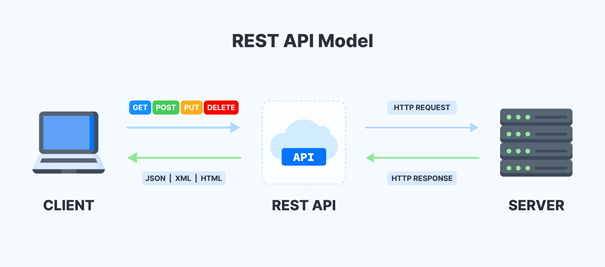
\includegraphics[scale=0.9]{sections/cloud-computing/images/rest-api.png}
    \caption{Funktionsweise von REST}
    \label{fig:ai-builder-tagging-figure}
\end{figure}

Stabile und interaktive Anwendungen setzten voraus, dass Programme untereinander barrierefrei kommunizieren können. Eine API, Application Programming Interface, definiert Regeln, die diese Kommunikation erleichtert. Unter diesen Programmen kann man entweder Softwarebibliotheken, ein Betriebssystem oder einen Webserver verstehen.
Der entscheidende Vorteil von API ist, dass das anfragende Programm keinerlei Informationen über das dahinterstehende System des Antwortgebers haben muss.

\textbf{REST-API}: Einer der bekanntesten Architekturen einer API ist REST. Representational State Transfer ist ein Stil für die Entwicklung von Anwendungen, die untereinander auf irgendeine Weise vernetzt sind. Es wird oft für die Entwicklung von Web-APIs verwendet.
Wichtig zu wissen ist, dass REST zustandslos ist. In diesem Kontext bedeutet zustandslos, dass Anfragen des Clients alle notwendigen Informationen für den Server besitzen muss. Der Client kann beispielsweise nicht davon ausgehen, dass sich der Server an die vorherigen Requests des Clients erinnern kann.
REST-APIs senden im Normalfall HTTP-Anfragen wie GET, POST, PUT, etc.

    \item Ein \textbf{Software Development Kit}, kurz SDK, ist eine Sammlung aus mehreren Tools, die von einem Hersteller einer Programmiersprache, eines Betriebssystems oder einer Hardwareplattform zur Verfügung gestellt werden. Diese Tools können Debugger, Frameworks oder eine Sammlung aus Codebibliotheken sein.
\end{enumerate}

\subsection{Cognitive Computing}

Cognitive Computing ist ein intelligentes System, das durch umfangreiches Lernen und zielgerichtetes Denken mit Menschen in ihrer natürlichen Form spricht, und diese nachahmt. Cognitive Computing ist die dritte Ära der Informatik. Gleichzeitig hat Cognitive Computing sowohl in der Wissenschaft als auch in der Industrie breite Aufmerksamkeit auf sich gezogen. Die Kombination aus maschineller und menschlicher Intelligenz kann die komplexesten Probleme der Welt lösen. Die Verarbeitung natürlicher Sprache mit Sentimentanalyse, künstlicher Intelligenz (KI), maschinellem Lernen und neuronalen Netzen, ist der Eckpfeiler von Cognitive-Computing-Prozessen, die Probleme wie Menschen lösen können. Heutzutage wenden fortschrittliche Technologien Cognitive Computing in vielen Bereichen an. Angesichts der heutigen Datenexplosion und der sich schnell ändernden Geschäftsumgebungen können kognitive Systeme intelligente, fließende und verbesserte Mensch-Maschine-Interaktionen effektiv angehen. Künstliche Intelligenz wird in vielen Anwendungen wie Alexa, dem Sprachassistenten von Amazon, Netflix und den Algorithmen von Amazon verwendet, um den nächsten Film oder Kauf vorzuschlagen. Die Weiterentwicklung dieser Technologie und ihre Übernahme im öffentlichen und privaten Sektor wird die Zukunft des Cognitive Computing aufgrund technologischer Entwicklungspfade und -trends stark beeinflussen. Kognitive Systeme müssen in Geschäfts- und breiten Anwendungen anpassungsfähig, interaktiv, zustandsbehaftet und kontextbezogen sein. Zu den Anwendungen, die von solchen Technologien mit Cognitive Computing profitieren können, gehören Finanz- und Investmentfirmen, Gesundheitswesen, Reisen und Tourismus, ebenso Gesundheit, Bildung und Lernen, Landwirtschaft, sowie Kommunikations- und Netzwerktechnologie.

\subsection{Cognitive Computing und Cloud Computing}

Cloud Computing virtualisiert die Datenverarbeitung, den Speicher und die Bandbreite. Dadurch werden die Kosten für die Bereitstellung von Softwarediensten gesenkt und die Industrialisierung, sowie die Förderung der Anwendung des Cognitive Computings unterstützt. Darüber hinaus bietet die hohe Rechen- und Speicherkapazität des Cloud Computing dynamische, flexible, virtuelle, gemeinsam genutzte und effiziente Rechenressourcendienste für das Cognitive Computing.

Nachdem die Big-Data-Analyse auf der CC-Plattform durchgeführt wurde, werden Technologien wie maschinelles Lernen eingesetzt, um Daten zu analysieren und die Ergebnisse in verschiedenen Bereichen anzuwenden. Die verschiedenen Kategorien von Informationen entsprechen unterschiedlichen Verarbeitungstechnologien. So entsprechen beispielsweise die wörtlichen Informationen der natürlichen Sprachverarbeitung und die bildlichen Informationen dem maschinellen Sehen. Der kognitive Dienst von IBM für Sprache und die kognitive Computing-Anwendung von Google legen den Schwerpunkt auf die Verwirklichung von gehirnähnlicher Wahrnehmung und Urteilsfähigkeit durch den Einsatz eines Cloud-Service-Modells, um präzise Entscheidungshilfen zu bieten. Cloud Computing und das Internet of Things (IoT) bieten eine Software- und Hardwarebasis für Cognitive Computing, während die Big-Data-Analyse Methoden und Denkweisen zur Entdeckung und Erkennung neuer Möglichkeiten und neuer Werte in Daten bereitstellt.
